\chapter[EFS Calculations]{Interatomic Potential: Energy, Force Stress Calculations}
\label{chap:appendix-activity-v2}

\FloatBarrier
\subsection{Calculating Energy, Force and Stress}
\label{section:backgroundenergyforcestress}

Molecular dynamics simulations do not need to include the weak or strong force, and the gravitational forces between atoms in the simulated material are so weak in comparison to the electromagnetic force, they can also be ignored.  There is a force between all the atoms within a real material, but the electromagnetic force is inversely proportionally to the separation of the atoms.  Above a certain separation, the electromagnetic force can also be ignored, in order to simplify the computation.

\FloatBarrier
\subsubsection{Neighbour List}
\label{section:neighbourlist}

A cut off radius can be introduced to limit the number of neighbours (section \ref{section:tendingtozero}).  As the lattice parameter decreases, the atoms are brought closer together, and as the cut off radius is increased more atoms are considered to be within the sphere of influence of one another.  Both increase the number of neighbours each atom has (fig. \ref{fig:nlsize}).

\begin{figure}[tbp]
  \begin{center}
    \includegraphics[scale=0.40]{chapters/interatomic_potential_fitting/plots/atom_neighbours.eps}
    \caption{Neighbouring atom count dependant upon lattice parameter and cutoff radius}
    \label{fig:nlsize}
  \end{center}
\end{figure}

Building a neighbour list may take a long time, depending on the parameters.  If a simplistic approach is taken, for N atoms in the supercell, there will be approximately $27N^2$ checks between atoms to see whether they are within the cut off radius of one another.  For larger numbers of atoms in a supercell, the whole may may be decomposed into smaller domains.

For example, a 16x16x16 FCC supercell, containing 16,384 atoms, would require looping $27 \times 16,384^2 = 7.25 \times 10^9$ times.  Breaking the supercell into 64 smaller domains with 256 atoms in each, reducing the problem to $64 \times 27 \times 256^2 = 1.13 \times 10^8$ loops.

For this work, the supercells used to calculate bulk properties from the interatomic potentials, and the configurations generated by \acrshort{dft}, contain fewer than 1,000 atoms, removing the need to decompose the configuration into smaller sub cells.

\begin{figure}[tbp]
  \begin{center}
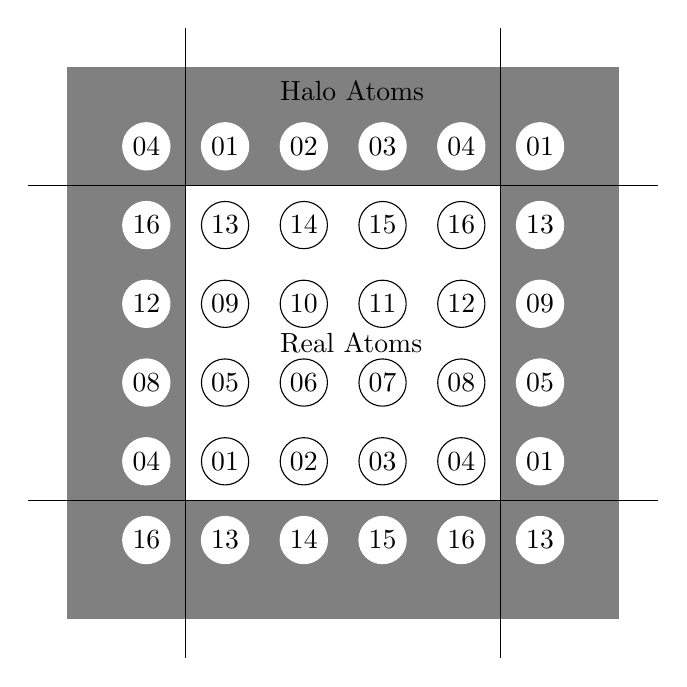
\begin{tikzpicture}
\filldraw [gray] (0.5,0.5) -- (0.5,7.5) -- (7.5,7.5) -- (7.5,0.5) -- (0.5,0.5);
\filldraw [white] (2.0,2.0) -- (2.0,6.0) -- (6.0,6.0) -- (6.0,2.0) -- (2.0,2.0);
\draw (0,2) -- (8,2);
\draw (0,6) -- (8,6);
\draw (2,0) -- (2,8);
\draw (6,0) -- (6,8);
\draw (2.5,2.5) circle [radius=0.3] node {$01$};
\draw (3.5,2.5) circle [radius=0.3] node {$02$};
\draw (4.5,2.5) circle [radius=0.3] node {$03$};
\draw (5.5,2.5) circle [radius=0.3] node {$04$};
\draw (2.5,3.5) circle [radius=0.3] node {$05$};
\draw (3.5,3.5) circle [radius=0.3] node {$06$};
\draw (4.5,3.5) circle [radius=0.3] node {$07$};
\draw (5.5,3.5) circle [radius=0.3] node {$08$};
\draw (2.5,4.5) circle [radius=0.3] node {$09$};
\draw (3.5,4.5) circle [radius=0.3] node {$10$};
\draw (4.5,4.5) circle [radius=0.3] node {$11$};
\draw (5.5,4.5) circle [radius=0.3] node {$12$};
\draw (2.5,5.5) circle [radius=0.3] node {$13$};
\draw (3.5,5.5) circle [radius=0.3] node {$14$};
\draw (4.5,5.5) circle [radius=0.3] node {$15$};
\draw (5.5,5.5) circle [radius=0.3] node {$16$};
\filldraw [white] (1.5,1.5) circle [radius=0.3] node [text=black] {$16$};
\filldraw [white] (1.5,2.5) circle [radius=0.3] node [text=black] {$04$};
\filldraw [white] (1.5,3.5) circle [radius=0.3] node [text=black] {$08$};
\filldraw [white] (1.5,4.5) circle [radius=0.3] node [text=black] {$12$};
\filldraw [white] (1.5,5.5) circle [radius=0.3] node [text=black] {$16$};
\filldraw [white] (1.5,6.5) circle [radius=0.3] node [text=black] {$04$};
\filldraw [white] (2.5,6.5) circle [radius=0.3] node [text=black] {$01$};
\filldraw [white] (3.5,6.5) circle [radius=0.3] node [text=black] {$02$};
\filldraw [white] (4.5,6.5) circle [radius=0.3] node [text=black] {$03$};
\filldraw [white] (5.5,6.5) circle [radius=0.3] node [text=black] {$04$};
\filldraw [white] (6.5,6.5) circle [radius=0.3] node [text=black] {$01$};
\filldraw [white] (6.5,2.5) circle [radius=0.3] node [text=black] {$01$};
\filldraw [white] (6.5,3.5) circle [radius=0.3] node [text=black] {$05$};
\filldraw [white] (6.5,4.5) circle [radius=0.3] node [text=black] {$09$};
\filldraw [white] (6.5,5.5) circle [radius=0.3] node [text=black] {$13$};
\filldraw [white] (6.5,1.5) circle [radius=0.3] node [text=black] {$13$};
\filldraw [white] (2.5,1.5) circle [radius=0.3] node [text=black] {$13$};
\filldraw [white] (3.5,1.5) circle [radius=0.3] node [text=black] {$14$};
\filldraw [white] (4.5,1.5) circle [radius=0.3] node [text=black] {$15$};
\filldraw [white] (5.5,1.5) circle [radius=0.3] node [text=black] {$16$};
\node[text width=3cm] at (4.7,7.2) {Halo Atoms};
\node[text width=3cm] at (4.7,4.0) {Real Atoms};
\end{tikzpicture}
\end{center}
\caption{A 2D representation of atoms in simulation box with a halo of atoms at the boundary}
\label{fig:nlatomshalo}
\end{figure}



To build the neighbour list a halo configuration is created such that it lies on top of the real atoms, but extends at least as far as the cut off radius on each side of the real simulation box (fig. \ref{fig:nlatomshalo}).  Periodic boundary conditions are used to construct the halo.

Once the halo list is computed, the neighbour list may also be computed by looping through the real atoms and halo atoms.  A simple pseudo coded sub routine is given (listing \ref{listing:halfneighbourlist}).

\FloatBarrier
\begin{lstlisting}[style=sFortran,caption={Simple subroutine for generating a half size neighbour list},label={listing:halfneighbourlist}]

! real_atoms - array holding coordinates of all real atoms
! halo_atoms - array holding coordinates of all halo atoms
! real_ids - unique id for each atom
! halo_ids - unique atom ids for halo atoms
! nlist_ids - array to store ids
! nlist_r - array to store separation

! Define the cutoff and counter start value
r_cut = 5.0
nl_counter = 1

! Calculate square
r_cut_sq = r_cut ** 2

! Loop over all real atoms
DO n_real = 1, real_atom_count
  ! Loop over all halo atoms
  DO n_halo = 1, halo_atom_count
    IF (real_ids(n_real) .LT. halo_ids(n_halo)) THEN
      r(1:3) = halo_atoms(n_halo, :) - real_atoms(n_real, :)
      r_sq = SUM(r(1:3) * r(1:3))
      IF (r_sq .LE. r_cut_sq) THEN          
        r_mag = sqrt(r_sq)          
        nlist_ids(nl_counter, 1) = real_ids(n_real)
        nlist_ids(nl_counter, 2) = halo_ids(n_halo)        
        nlist_r(nl_counter, 1) = r_mag
        nlist_r(nl_counter, 2:4) = r(1:3)/r_mag
        nl_counter = nl_counter + 1
      END IF
    END IF
  END DO
END DO 
\end{lstlisting}

The resulting list will contain unique a pair combinations; i.e. the pair atom 1 and atom 2 will only be recorded once, and not also as atom 2 and atom 1.

Many modern \acrshort{md} codes are designed to run on computers with many thousands of processor cores.  This leads to a choice of approaches, either to keep the configuration in shared memory and allow multiple processes to work on the same data, or break the data up, distributing it across various nodes.    

In the case of DL\_POLY a link-cell domain decomposition is used\cite{dlpolymanual}.  The supercell is divided up into subcells, and these must be at least the size of the cut-off radius.   Each processor will work on a geometric domain and these will only interact with their immediate neighbours.  The halo data for each subcell is only passed between processors before and after the calculation of the equations of motion of the atoms within each subcell.

\begin{figure}[!htbp]
  \begin{center}
    \includegraphics[width=.6\linewidth]{chapters/interatomic_potential_fitting/images/domain-decomp.png}
    \caption{Partitioning in \acrshort{lammps}\cite{lammpsdd}}
    \label{fig:lammpsdd}
  \end{center}
\end{figure}

This is also the approach used by the \acrshort{lammps} code.  The simulation is partitioned into either boxes where the density of atoms is uniform or tiles where there are regions with few or no atoms (fig. \ref{fig:lammpsdd}).  This ensures processors are evenly utilised.




\FloatBarrier
\subsubsection{Computing Total Energy}

The total energy of the system is the sum of the individual energies for the atoms in the simulation.  The type of atom (or pairs of atoms) will determine which function is used.

First, to compute the pair potentials:

\begin{itemize}
\item set the total energy of the system equal to zero
\item set the starting energy for each atom in the system to zero
\item loop through the atom pairs in the entire neighbour list
\item for each atom pair, A and B, use the known separation and the potential function to compute the potential energy on atom A due to B and vice versa
\item add this potential energy to both A and B
\item after looping through the neighbour list, add all the energies due to the pair potential to the total energy
\end{itemize}

For an EAM or 2BEAM potential, the densities and embedding energies must also be computed:

\begin{itemize}
\item set the electron density at the position of (for each) atom to zero
\item loop through the atom pairs in the entire neighbour list
\item for each atom pair, using the density function for the atom A, the density at atom B due to atom A will be calculated and added to the density at atom B
\item if the atoms are both of the same type the same density will be added to atom A due to atom B
\item if the atom types are different, using the density function for the atom B, the density at atom A due to atom B will be calculated and added to the density at atom A
\item following looping through the neighbour list, to calculate the densities at each atom, the list of atoms will be looped through
\item for each atom, the density value at the position of that atom, will be input into the appropriate embedding function to calculate the embedding portion of the energy
\item add all the embedding energies to the total energy of the system
\end{itemize}

For a 2BEAM potential, repeat the above procedure for the second group of density functions and embedding functions (do not repeat calculation of the pair potentials).


\subsubsection{Computing Forces on Atoms}

In order to calculate the forces on the atoms with an \acrshort{eam} or \acrshort{2beam} potential, the neighbour list and atom list will need to be looped through several times.  First, the pair potential and force due to the pair potential must be calculated by a complete loop through the neighbour list.  At the same time, the density at each atom location is also calculated.  The embedding energy may then be computed by looping through all the atoms and using the electron density at each atom to give the energy of the atom embedded in that density.  The third and final loop will run through the neighbour pairs in the neighbour list once more computing the force on each atom due to its embedding in the electron background.

\begin{equation}
\begin{split}
F^k_{pair} = -\sum \limits_{j=1, j \ne k}^{N} \frac{\partial V_{kj} (r_{kj}}{\partial r_{kj}} \frac{\vec{r}_{kj}}{\lvert\vec{r}_{kj}\lvert} \\
F^k_{embed} = -\sum \limits_{j=1, j \ne k}^{N} \left(\frac{\partial F}{\partial \rho_k} \frac{\partial \rho (r_{j})}{\partial r_{kj}} + \frac{\partial F}{\partial \rho_j} \frac{\partial \rho (r_{k})}{\partial r_{kj}} \right)  \frac{\vec{r_{kj}}}{r_{kj}}
\end{split}
\label{eq:computingForces}
\end{equation}

The force on each atom, due to surrounding atoms, may be split into two; force due to the pair potential, and the force due to the embedding of the atom (eq. \ref{eq:computingForces})\cite{dawbaskeseam}\cite{dlpolymanual}.


\subsubsection{Computing Stress}

The stress is to be calculated assuming the system is at 0K\cite{wikivirialstress} so the virial stress equation is eq. \ref{eq:eqVirialStress}.

\begin{equation}
\begin{split}
\tau_{ij} = \frac{1}{2 V} \sum_{k,l \in V} \left({x_i}^{(l)} - {x_i}^{(k)} \right) {f_j}^{(kl)}
\end{split}
\label{eq:eqVirialStress}
\end{equation}

Within the computer code, the individual force components between pairs of atoms are stored as well as an equal sized array of vectors representing their spatial separation.  Those pairs with one atom in the halo around the simulation box are used to calculate the stress on the simulation box.


\subsubsection{Pseudo Code for the Energy, Force and Stress Subroutine}

The calculation requires several arrays to temporarily store data.  The electron densities and gradients of the density function are stored for multiple groups of densities and embedding functionals.  The overall forces on each atoms also need to be stored as well as the force between pairs of atoms, as this is required to compute the virial stress.  The Fortran code to compute this is included in the appendix (section \ref{section:appendixenergyforcestress}) and a pseudocode in listing \ref{listing:efscalc} explains the process.

\begin{lstlisting}[style=sFortran,caption={Pseudo Code for Energy and Stress Force Calculation}, label={listing:efscalc}]

electron_density[1:n_atoms, 1:bands] = 0.0  ! electron density at each atom
energy = 0.0                                ! total energy
forces[:,:] = 0.0                           ! forces each atom, 3D
force_between_pairs[:,:] = 0.0              ! used to store force between pairs, for stress computation
stress[:,:] = 0.0D0

! LOOP 1 - Pair energy, force and calculate densities
DO n = 1, neighbour_count
  E = get_PairEnergy(atom_a, atom_b, r[n,:])
  F[:] = get_PairForce(atom_a, atom_b, r[n,:])

  ! Save energy
  energy = energy + E

  ! Save Force
  f[atom_a, :] = f[atom_a, :] - F[:]
  f[atom_b, :] = f[atom_b, :] + F[:]
  force_between_pairs[:,:] = force_between_pairs[:,:] - F[:]   // Used to calculate stress
  
  ! Loop through density bands
  DO band = 1, bands
    ! Electron density at A due to atom B
    electron_density[atom_a, band] = get_Density(atom_b, r)
  
    ! Electron density at B due to atom A
    electron_density[atom_b, band] = get_Density(atom_a, r)
  END DO
END DO

! LOOP 2 - Embedding energy
DO n = 1, atom_count
  ! Loop through density bands
  DO band = 1, bands
    energy = energy + get_EmbeddingEnergy(n, band)
  END DO
END DO

! LOOP 3 - Embedding force
DO n = 1, neighbour_count
  ! Loop through density bands
  DO band = 1, bands
    dgradA = get_DensityGradient(atom_b, r, band)
    dgradB = get_DensityGradient(atom_a, r, band)
    fgradA = get_EmbeddingGradient(atom_a, electron_density[atom_a, band])
    fgradB = get_EmbeddingGradient(atom_b, electron_density[atom_b, band])

    F[:] = (fgradA * dgradB + fgradB * dgradA) * r[n, :]

    f[atom_a, :) = f(atom_a, :) - F[:] 
    f(atom_a, :) = f(atom_a, :) + F[:] 
    
    force_between_pairs[n,:] = force_between_pairs[n,:] - F[:]   // Used to calculate stress
  END DO
END DO

! LOOP 4 STRESS
DO n = 1, neighbour_count
  ! Only compute if the second atom is in the halo 
  IF(nlisthalo(n))THEN  
    DO i = 1,3
      DO j = 1,3
        stress[i,j] = stress[i,j] + (r[n, i] * force_between_pairs[n,j])
      END DO
    END DO
  END IF
END DO
stress[1:3, 1:3] = stress[1:3, 1:3] / (2.0 * volume)

\end{lstlisting}